% Chapter 1

\chapter{Introduction} % Main chapter title
\label{chapter1} % For referencing the chapter elsewhere, use \ref{Chapter1} 

\section{Purpose/Motivation}
The elderly population is in a constant rise, currently 15\% of the Norwegian population is above the age of 65. By the turn of the century the elderly population is expected to double \cite{elder}. The initial rise of the elder population will be most noticeable in those below the age of 80, as seen in figure \ref{fig:elderPopulation}. After 2025 a great increase in the population above the age of 80 is expected. The Norwegian Institute of Public Health* reports that two out of three above the age of 75 consider themselves having ``good health'' but only a third preserve this level of health until death \cite{elder}.

\begin{figure}[h!]
	\centering	
		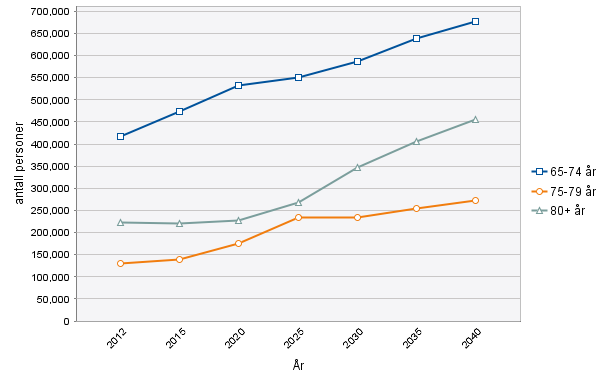
\includegraphics[width=0.5\textwidth]{eldrevekst.png}
		\caption{\footnotesize Elder population estimation \cite{elder}}
		\label{fig:elderPopulation}
\end{figure}
In 2010 one of the largest ever systematic efforts to describe the global health situation was conducted. The article was later published in The Lancet \cite{globalBurden}. One of their many findings was that since 1970 men and women have gained an additional ten years to their life expectancy, but spend more time living with injuries and illness. %KOMMER TILBAKE HIT

In the late 1990s the Norwegian statistical bureau* published a paper predicting a major increase in the elderly population \cite{eldreEksplosjon}. The working population compared to the retired currently holds a ratio of 5 to 1. This is expected to drop below 3 by the year 2040. Because of this, the greatest challenges within welfare are expected to occur between 1998 and 2020. 

With such predictions the Norwegian government formed a committee (referred to as Hagen-utvalget*) that would investigate the current situation and suggest solutions for accommodating the increase in the percentage of elderly \cite{haagen}. One of the conclusions in the report was that too little of today's technology is incorporated as welfare technology* for the elderly. A Danish report refereed to by Hagen-utvalget* states that around 20\% of the tasks performed by healthcare personnel could be completely or partly replaced by technology \cite{kmd}. 

To handle the rising percentage of elderly, Hagen-utvalget* suggest a national three step program that focuses on using welfare technology to diminish falls, social isolation and cognitive failure. Thus improving the overall quality of life for the elder population as well as reducing the workload for health care personnel. Step 3 states that:
\begin{quote}
\textit{``Opt on technology that stimulates, activates and structures daily life.''}
\end{quote}
One way of using modern technology to reduce sedentary behaviour can be to through self-reflection using personal informatics tools such as the activPAL. %Does this work, I feel it's a little out of place...

The amount of time adults spend in a sedentary position has increased over the last 30 years. The reasons for this are many, but increased use of technology and ease of transport are one of the main factors \cite{sedentaryBehaviour}. An American study shows that 1 of 4 US adults spend 70\% of their waking hours in a sedentary position, 30\% in light activity, and little to no time is spent exercising.

In the last decade research has started to emerge that links extended periods of sedentary time to metabolic risks\cite{sedentaryTime}, obesity, and abnormal glucose metabolism \cite{breaksSedentary}. It is suggested that prolonged periods of sedentary time should be avoided by increasing the number of breaks during sedentary time, and these findings suggest new public health recommendations \cite{breaksSedentary}. Another study goes as far as stating that prolonged sedentary time is strongly related to metabolic risks independent of physical activity \cite{sedentaryActivity}, and that older people benefit more from reducing the sedentary time. What has not been shown by research is how long a subject can stay sedentary before it has negative impact on the individuals health, or how long the breaks between sedentary time should be.

Personal Informatics* has become an emerging branch of technology to help individuals collect personal information for the purpose of self-reflection and self-monitoring. We will look relevant trends and technology later in this project. By using personal data and visualize their patterns we hope to bring awareness to their activity levels, and identify periods of long sedentary time. 

\section{Project context/Thesis Scope}
This project is a cooperation between the Department of Computer and Information Science (IDI)* at the Norwegian University of Science and Technology (NTNU) and St. Olavs University Hospital in Trondheim. The project...

\section{Research questions}

\section{Research method}

\section{Thesis outline}
